\chapter{Teaching a Robot to Support Child Learning}\label{chap:tutoring}
\glsresetall
\graphicspath{{images/tutoring/}}

\begin{framed}
	\textbf{Key points:}
	
	\begin{itemize}
		\item Design of an experiment to test \acrshort{sparc} in an educative application with children.
		\item Design and use of a new learning algorithm adapted from nearest neighbours to teach quickly and efficiently in an online fashion.
		\item Between participant study involving 75 children compared 3 conditions: a passive robot, a supervised robot and an autonomous robot.
		\item Psychology PhD student taught the supervised robot using \acrshort{sparc}.
%		\item No significant differences of child learning between conditions.
		\item Children interacted similarly with the autonomous and supervised robot, but differently with the passive robot.
		\item Demonstration of the applicability of \acrshort{sparc} to teach a robot online an action policy to interact with humans.
	\end{itemize}
\end{framed}

Parts of the work presented in this chapter have been published verbatim in \cite{senft2017toward}, additional publications are under review \footnote{Note about technical contribution in this chapter: the author extended code the freeplay sandbox, see \url{https://github.com/freeplay-sandbox/} and forks.}. The final publications are available from AAAI, EPFL via:
\begin{itemize}
	\item \url{https://aaai.org/ocs/index.php/FSS/FSS17/paper/view/16011}.
	\item \url{https://r4l.epfl.ch/files/content/sites/r4l/files/HRI2018/proceedings_2018/paper4.pdf}
\end{itemize} 

\newpage

\section{Motivation}

Chapters \ref{chap:woz} and \ref{chap:control} tested the \gls{sparc} in interactions between robots or in a virtual world but not for human-robot interactions as it was intended to used for. As such, this Chapter addresses the thesis of the research work and evaluates if \gls{sparc} can efficient be used to teach a robot an interactive behaviour in a real human-robot interaction. \gls{hri} in the wild are typically constrained but underspecified environment where social behaviour play an important role. This study takes place in the framework of robot tutors for children in education. Tutoring offers a rich and complex interaction between the child and robot and as such is a good example of typical \gls{hri}. The scenario and the code is based on \cite{lemaignan2017free} but have been adapted to provide the teaching task, the testing of knowledge, the robot controller, the learning algorithm and the interface with the teacher.

This study aims to explore if \gls{sparc} can be used to teach a robot an efficient action policy. As such, three conditions have been compared: a passive robot (not providing any support), a supervised robot (learning from a human teacher and supporting the child) and an autonomous robot (applying the learned behaviour). These three conditions, with the passive robot as a control condition, allow us to study both the teaching process and the efficiency of the taught behaviour when being executed without supervision.

\section{Scope of the Study}
%Might need to go in method??
\subsection{Setup of the study}

Similarly to the study presented in Chapter \ref{chap:woz}, this study is based on the Sandtray paradigm
\citep{baxter2012touchscreen}: a child interacts with a robot through a large touchscreen located between them.
Additionally, a teacher can use a tablet to control the robot in one of the conditions (cf. Figure
\ref{fig:tutoring_setup}). This type of potentially triadic interaction is typical to the interactions we considered when framing this research (cf. Figure \ref{fig:intro_setup}). We desire an efficient behaviour for the robot in the application interaction (i.e. child tutoring) and a human teacher has knowledge about how the robot should behave and can transfer it to the robot in situ by using \gls{sparc}.

\begin{figure}[ht]
	\centering
	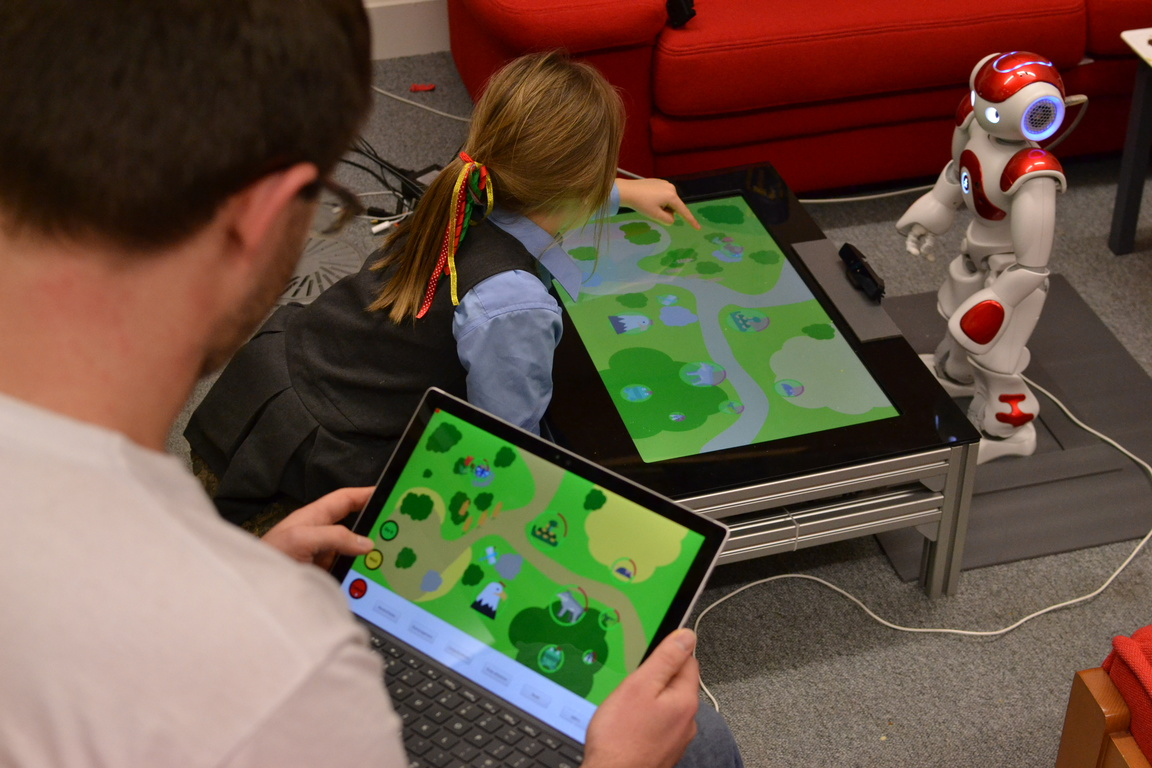
\includegraphics[width=.5\textwidth]{setup.jpg}
	\caption{Setup used in the study: a child interacts with the robot tutor, with a large touchscreen sitting between them displaying the learning activity; a human teacher provides guidance to the robot through a tablet and monitors the robot learning.}
	\label{fig:tutoring_setup}
\end{figure}

By interacting with the robot and the sandtray, the child is expected to gain knowledge on a specific topic. For this study, the task is learning about food chains, by exploring a specific food web (interconnections between multiple food chains). To achieve this, children played a game on the sandtray where they could move animals and discover interaction between them. Learning was evaluated by test before, after and between the sessions. The robot guided the child through the study and could, depending of the condition, support the child during the game.

\subsection{Food Chain Game}

The main learning activity teaching the children the food web is a game composed of ten animals and three types of plants. Animals have energy decreasing over time and they have to eat to stay healthy. Animals are immobile unless the child or the robot moves them and eat or be eaten when entering in contact with another animal or a plant. Children have to feed animals by moving them to their food to give them more energy. By feeding the animals, children can learn what food each animal eats. Figure \ref{fig:tutoring_game} presents an example of the game screen in the middle of a session.

\begin{figure}[ht]
	\centering
		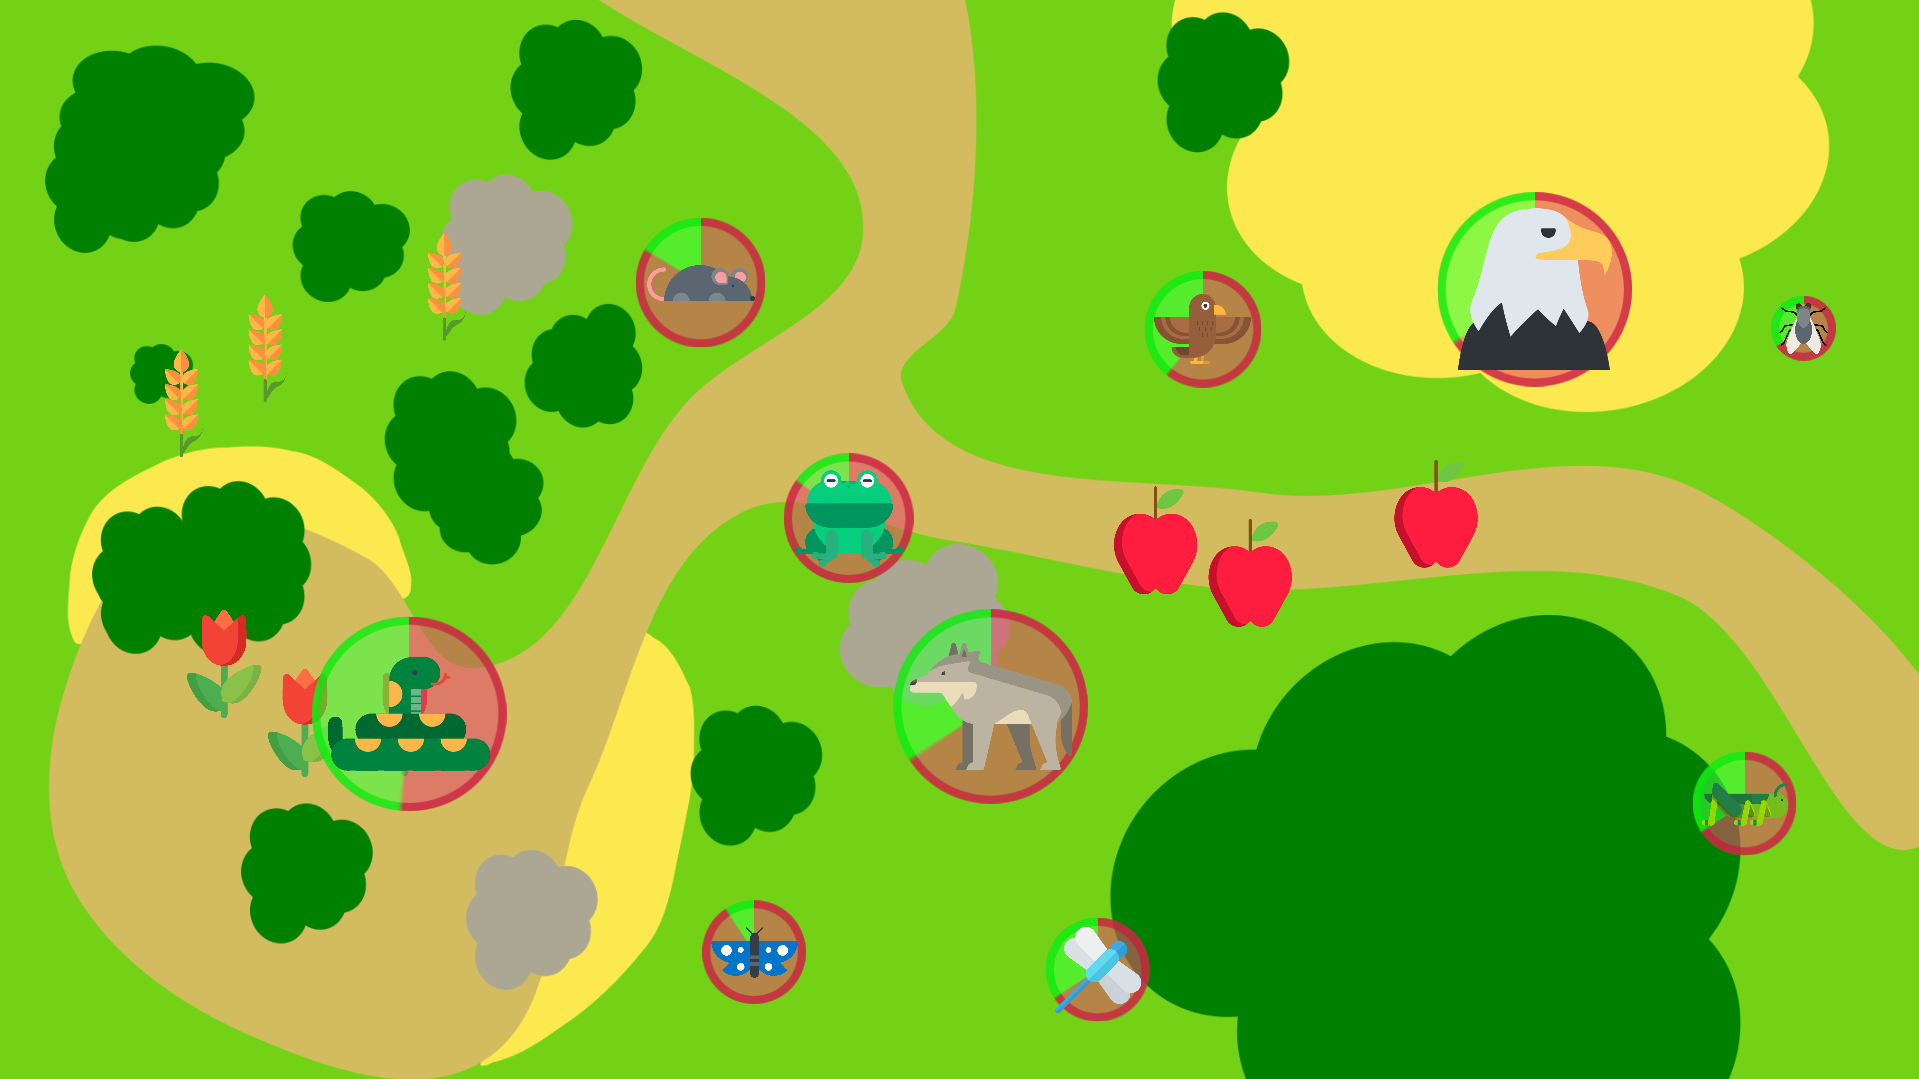
\includegraphics[width=1\textwidth]{game.png}
		\captionsetup{width=.9\linewidth}
		\caption{Example of the game. Animals have energy in green and have to eat plants of other animals to survive.}
		\label{fig:tutoring_game}
\end{figure}

\subsection{Robot Behaviour}
 
During the game, the robot can execute actions to provide hints and support to the child. The robot has access to five types of actions:
\begin{itemize}
	\item Movements: moving any animal to, toward or away from any items (animal or plant) - the robot points to an animal and moves it on the game while describing its action (e.g. "The eagle needs help getting close to the mouse").
	\item Drawing attention: the robot points an item and says a reminder to the child (e.g. "Don't forget the frog").
	\item Reminding rules: the robot says one of 5 sentences on the game (e.g. "Move the animals to feed them" or "Don't feed animals with a lot of energy").
	\item Congratulation: the robot provides congratulations (e.g. "Well done").
	\item Encouragement: the robot provides encouragement (e.g. "You can do it").
\end{itemize}

For each utterance joining an action, multiple versions are available, and a random one not used recently is selected. Considering all the possible combinations of actions and items, the total number of actions adds up 655.

These actions have been selected to represent different level of support, from general motivation and informations on the game to information about which animals the child should focus on or direct information about what animals eat. This selection of actions aims to cover a large range of possible tutoring behaviours humans could use. 

\subsection{Wizard of Oz Application}

The main aim of the study being testing \gls{sparc} in a real \gls{hri}, the teacher needs to communicate with the robot. To allow this interaction between the teacher and the robot, a \gls{gui} has been developed representing the current state of the game exactly as the child sees it on the touchscreen (as see in Figure \ref{fig:tutoring_gui}). This \gls{gui} runs on a tablet as it would allow teacher (or other robot users) to supervise and teach the robot while monitoring the application interaction. Buttons for the actions (excluding movements) allow the teacher to select which action the want the robot to execute. The teacher can also have the robot move animals simply by dragging and releasing animals' images on the tablet. The teacher can also select animals or plants to specify which action they intend to do. For instance, by clicking on the frog and the `Draw attention' button, the robot will execute the \textit{drawing attention to the frog}. Similarly, the moving action require two items: the animal moved and the target of the motion. By selecting a target before moving an animal, the teacher can be sure that the robot interpret the action correctly. This design of \gls{gui} gives access to the teacher to the full 655 actions without requiring as many buttons. Additionally, the selection of items is used by the robot controller to identify the relevant features to transmit to the algorithm for the learning.


\begin{figure}[ht]
	\centering
	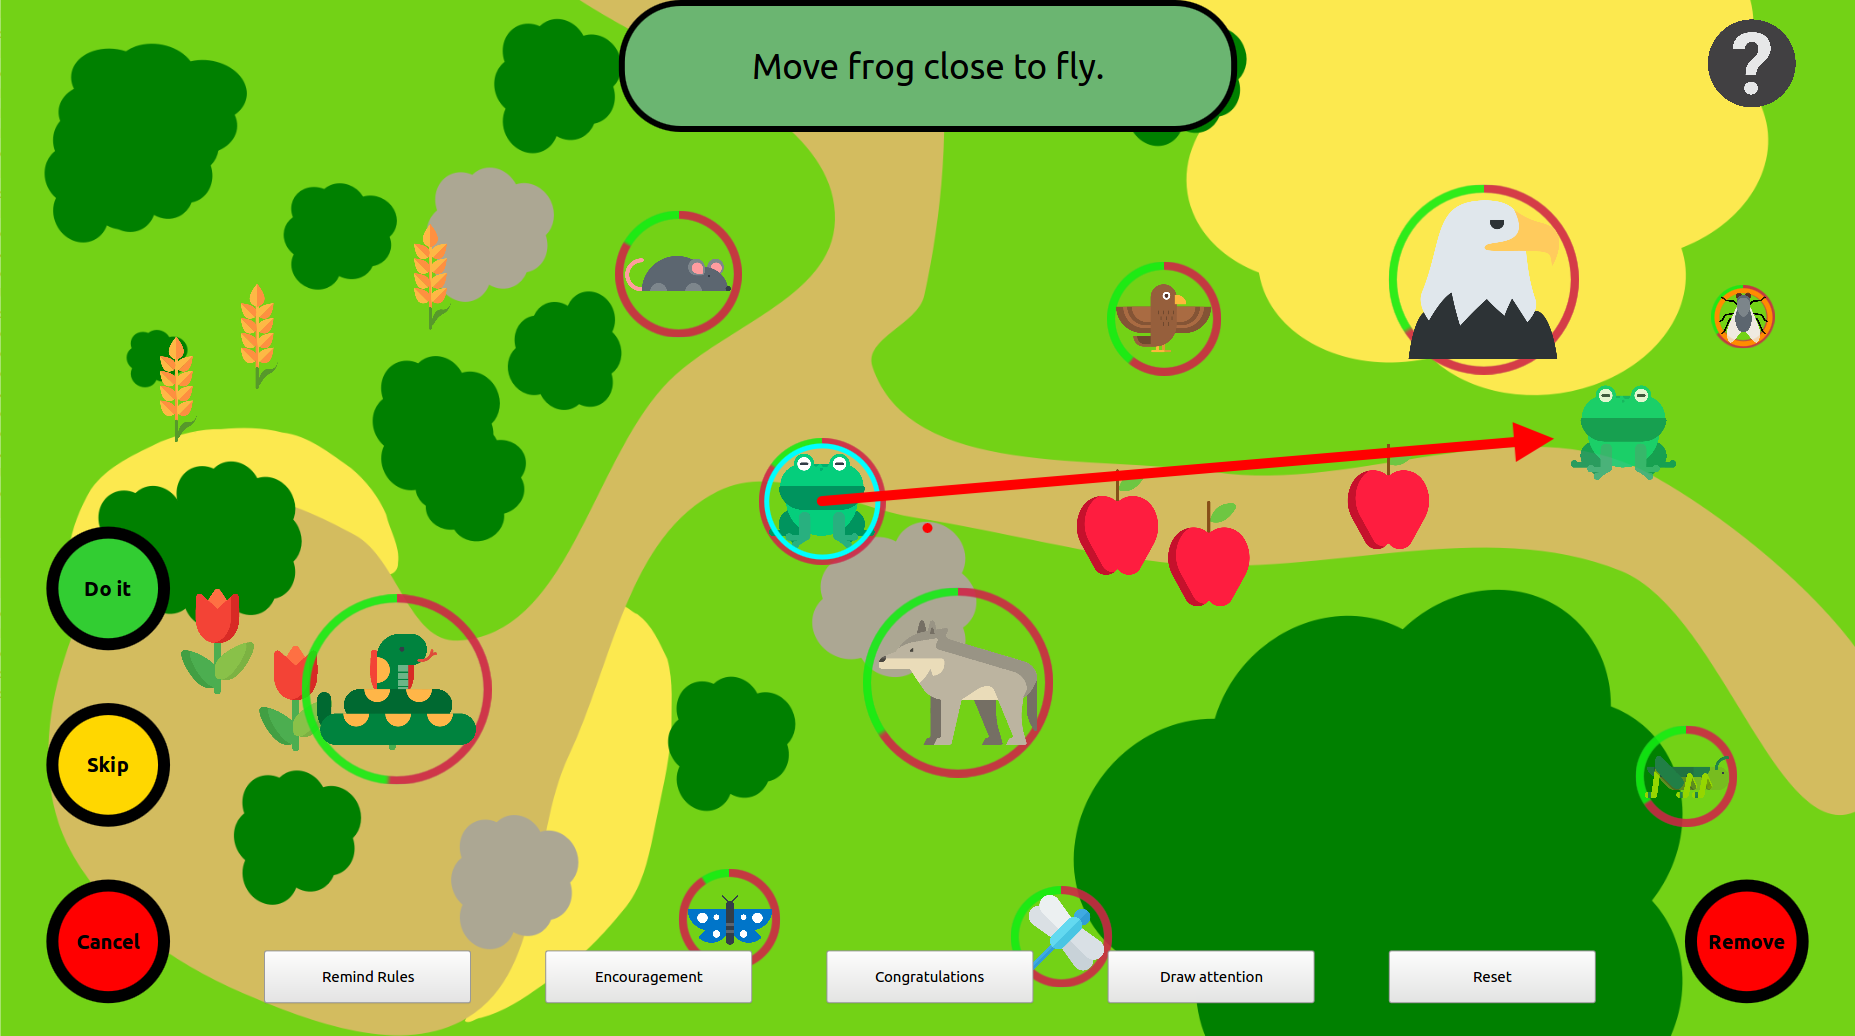
\includegraphics[width=1\textwidth]{gui.png}
	\captionsetup{width=.9\linewidth}
	\caption{\gls{gui} used by the teacher to control the robot and respond to its suggestions. The game presents the same state as in Figure \ref{fig:tutoring_game}, and he robot proposes to move the frog close to the fly (text bubble, arrow, moving the \textit{shadow} of the frog and highlight of the frog and the fly).}
	\label{fig:tutoring_gui}
\end{figure}


Finally, the \gls{gui} is also used by the teacher to respond to the propositions of the robot. Following the proposition of an action, a bubble describing the action will appear on top of the \gls{gui} and the corresponding items will be highlighted and if the action is a motion, an arrow will show the proposed motion. The teacher can react to the proposed action by pressing the "Do it", "Skip", "Cancel" or "Remove" buttons or let the action be executed. The action will be automatically executed after 2 seconds, during which the bubble will become greener to represent the passive acceptance of the action. The "Do it" button executes the action straight-away, the "Skip" button informs the algorithm that it should wait rather than doing the action, the "Cancel" button assigns a negative reward to this action in that case and finally, the "Remove" button looks for the closest previous instantiation of action in memory and removes it, preventing this instance to be executed later.

\subsection{Algorithm}

The learning algorithm's goal is to map an action (or no action) to each possible state. The state used in this study represents the situation of the game in a 210 dimensional vector, with value from 0 to 1. The dimensions include: distance between items, items' energy, time since events (child and robot touching each animal, robot's actions, interaction events: feeding an animal, death of animal...), progression in the game sessions and child face direction (toward the robot, the screen or away).

The actions and the state dimensions have been selected to be generic to many teaching task involving movable items: each item can have a value assigned to it (here energy, but this could be changed in other scenario), and some movable items (here animals) can be move toward or away from other items. Using these generic actions and this state definition, this implementation could be easily re-purposed to another teaching task.

The algorithm used for the learning is an adaptation of the one presented in \cite{senft2017toward}. It is an instance based algorithm similar to the nearest-neighbours algorithm \cite{cover1967nearest}. However, two differences are notable compared to the initial algorithm. Firstly, instead of being defined on the full state space, instances are defined on a sliced version of the state. The intuition is that states needed to cover complex action policy require large number of dimensions, however for a single action, large parts of the state are irrelevant: for example if a robot needs to pick-up a cup, the colour of the cup does not impact the optimal motion. For this implementation, when selecting actions, the teacher can highlight features of the environment which will \textit{activate} specific dimensions of the state space that are used to store the instance in memory. All \textit{non-activated} dimensions are left as wild-card. Then when comparing the current state to the saved instances, the distance is only computed on the \textit{activated} dimensions of the comparing instance. The second difference is that each instance saved has a reward assigned to it, if the teacher selected the action, a reward of $+1$ is assigned, and if the teacher cancelled the action (following an incorrect suggestion from the algorithm) a reward of $-1$ is assigned. When selecting an action, the algorithm looks through all the actions it have been using and for each action selects the closest instance and compute the expected reward as a multiplication of the distance with the reward assigned. Then the algorithm selects the action with the highest expected reward and proposes it if the value is higher than an adaptive threshold. 

The algorithm runs at 2Hz while we would expect actions to be selected every 5 to 20 seconds, so unlike most of the discrete cases of action selections, in most of the steps, no actions are required. To handle this difference of timescale, a waiting action have been added (through the ``skip button'') and an adaptive threshold only proposes actions with an expected reward higher than the threshold. Selecting an action can reduce the threshold, and cancelling or skipping an action can increase it. This adapts the rate of action propositions to the desires of the teacher. Another mechanism filters propositions from the algorithm not to transfer them to the teacher when an action is already proposed to the supervisor or the robot is acting and also rewards negatively impossible actions (such as moving dead animals).

\section{Methodology}

\subsection{Study Design}

Seventy-five children aged 8 to 10 participated in the study (age: \textit{M}=8.9, \textit{SD}=0.83; 11F/15M).  Children were first introduced to the robot and the aim of the interaction, then had a first pre-test to evaluate their initial knowledge. Before starting the teaching game, children have to complete a tutorial where they are introduced to the mechanics of the game: animals have life and have to eat to survive and children can move animals to make them interact with other animals or plants. After this short tutorial, they have to complete two sessions of the game where the robot can provide feedback and advices depending which conditions they are in. After these initial sessions of the game they have to complete a mid-test before playing another 2 sessions of the game and a last post-test before concluding the study. 

\begin{figure}[h]
	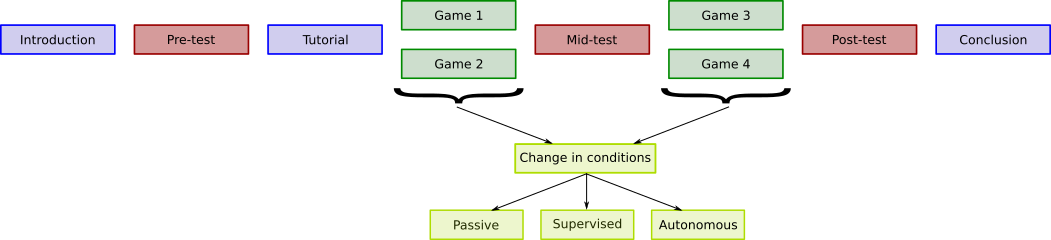
\includegraphics[width=.9\linewidth]{graph.png}
	\centering
	\caption{Methodology used for the study.}
	\label{fig:method}
\end{figure}

In all the conditions, the robot's behaviour during the introduction, tests, tutorial and conclusion is identical. The only change of behaviour happens during the games sessions. Figure \ref{fig:tutoring_game} shows an example of the game screen. The child can move 10 animals across the game field and can have them interact with other animals or plants. Animals lose energy over time and by interacting with their food the can regain some. Animals that are eaten lose a chunk of their life. The goal for the children is to keep animals alive as long as possible by feeding them and they earn stars representing how healthy their animals have been during the session. The game stops when 3 or more animals run out of energy and each game session lasted 1.6 minutes in average.

\subsection{Hypotheses}

\subsection{Metrics}
\subsubsection{Learning Evaluation}
During the pre-test, the experimenter demonstrate how to connect animals by drawing an arrow from the frog to the fly, and they removing the arrow by pressing the \textit{X} button. Then, children are asked to connect as many animals as possible. Figure \ref{fig:test} shows two examples of test, without or with all correct connections. When they think they are done, they can press the continue button, showing a screen asking confirmation to quit the test or give the opportunity to keep connecting animals. Additionally, the robot inform the child if not all the animals are connected to their food or that animal can eat many types of food if no more than one animal has been connected to two items. They are in total 25 different correct connections and 95 possible incorrect ones. As the child can connect as many arrows as desired, the performance is defined as the number of correct arrows above chance for the total number of connected arrows on the test divided by the maximum achievable performance to reach a score with a ceiling at 1.

\begin{figure*}[ht]
	\centering
	\begin{subfigure}[t]{0.5\textwidth}
		\centering
		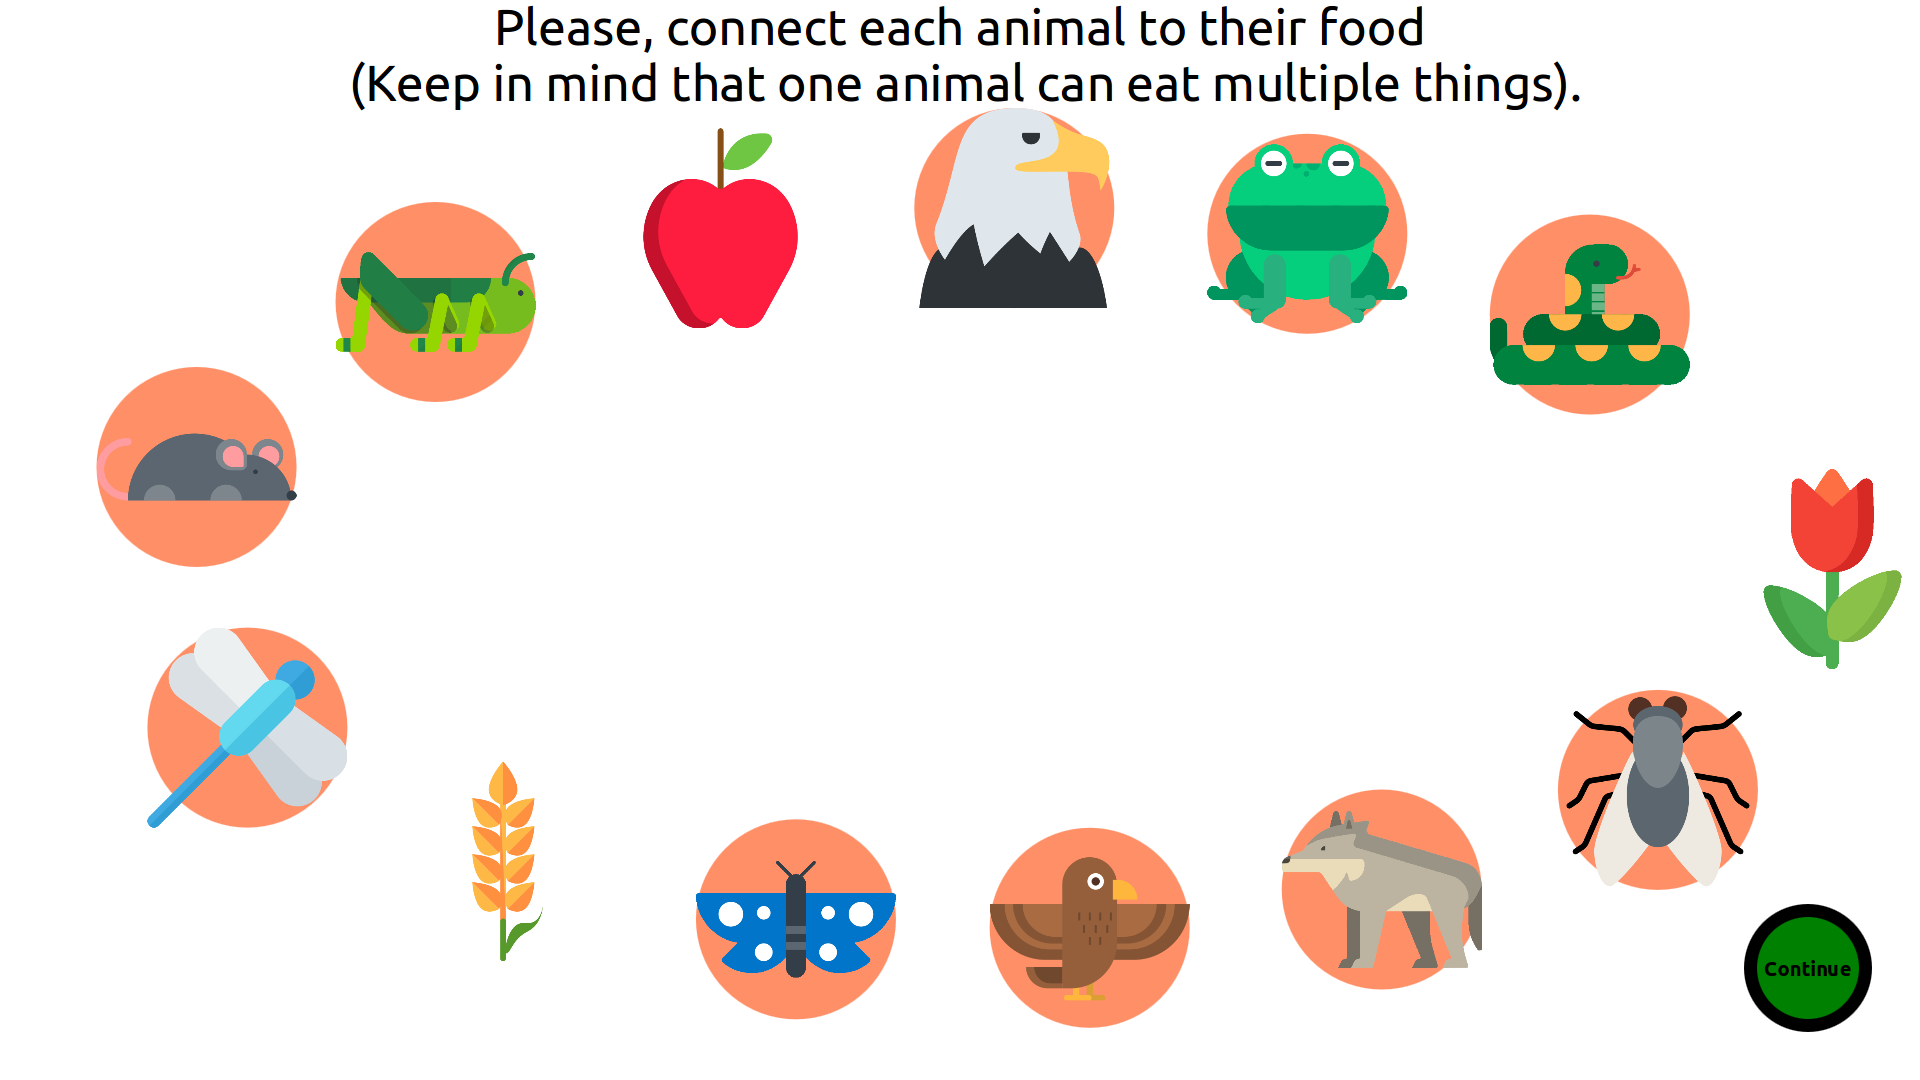
\includegraphics[width=0.95\textwidth]{empty_graph.png}
		\captionsetup{width=.95\linewidth}
		\caption{Empty screen that children face at each test. Red dots behind animals represent that they are not been connected to any food.}
		\end{subfigure}%
		~ 
		\begin{subfigure}[t]{0.5\textwidth}
			\centering
			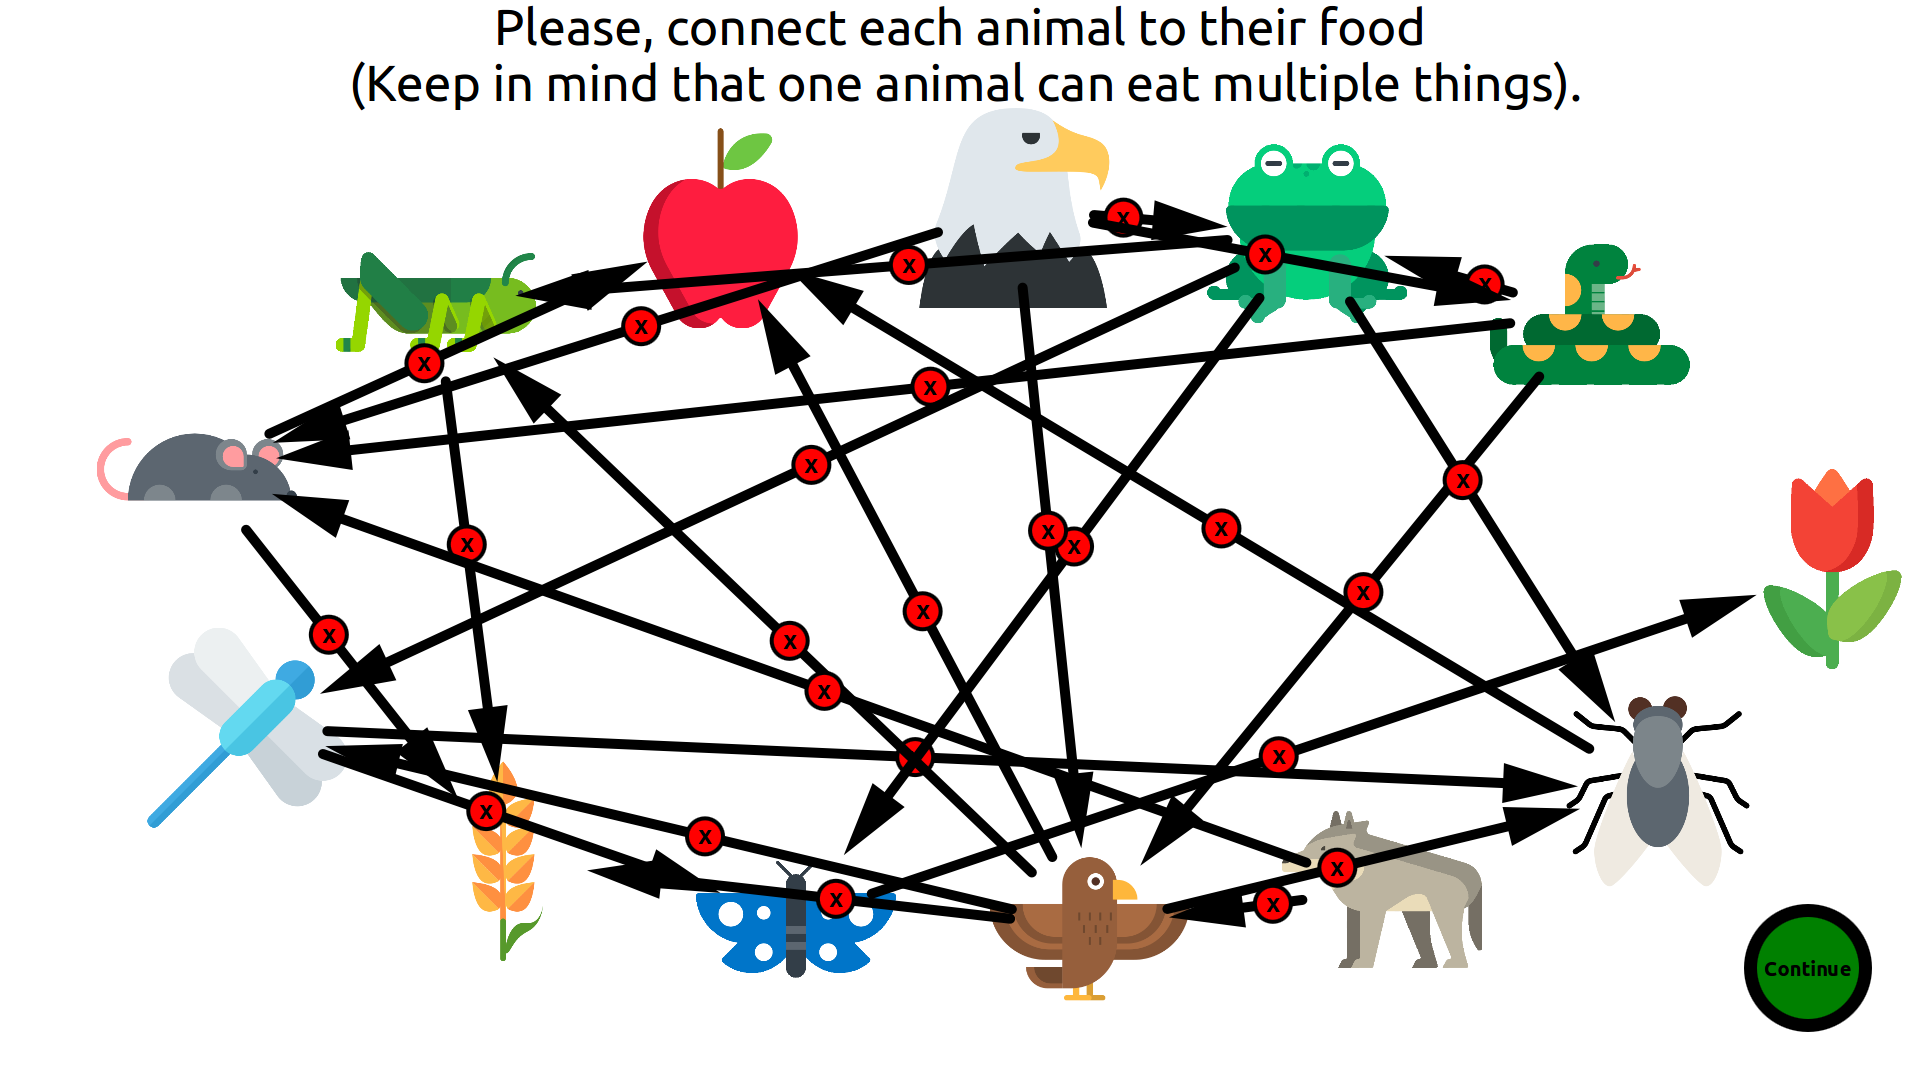
\includegraphics[width=0.95\textwidth]{full_graph.png}
			\captionsetup{width=.95\linewidth}
			\caption{Fully connected test with all the correct connections.}
			\end{subfigure}
			\caption{Test screen to evaluate children's knowledge, empty starting screen (a) and fully connected and correct test (b).}
			\label{fig:test}
			\end{figure*}
			
\section{Results}


To demonstrate the presence or the absence of effects, we used bayesian statistics on the data. As such the Bayes factor $B$ is reported and represents how much of the variance on the metric is explained by a parameter (if $B < 1/3$ there is no impact, if $B > 3$ the impact is strong, and if $1/3<B<3$ the results are inconclusive - \cite{jeffreys1998theory,dienes2011bayesian}). And the analysis is performed using the Jasp software \cite{jasp2018}.

%Preliminary results (currently in progress, due to be completed before the submission of the full article) show that (1) the robot is able to effectively jointly learn action and social policies (Figure 2), (2) the learning gains of the children supported by the autonomous robot are not significantly different from the gains when the learning is supported by a robot tele-operated by the human expert, which would indicate the utility of the approach.


\paragraph{Test Performance}

Figure \ref{fig:performance} shows the evolution of children's performance across the three tests. A Bayesian mixed-ANOVA show that in all conditions, children's performance increased across the tests ($B=1.5$x$10^{12}$), however the impact of the condition on the learning is inconclusive with a tendency to show no impact ($B=0.539$). This indicates that by being involved in the task, every children learned and improve their performances on the test (by gaining in average 13\% of the missing knowledge), but the robot behaviour during the game did not have an important impact on the children's learning gain (see Figure \ref{fig:learning}).

\begin{figure}[ht]
	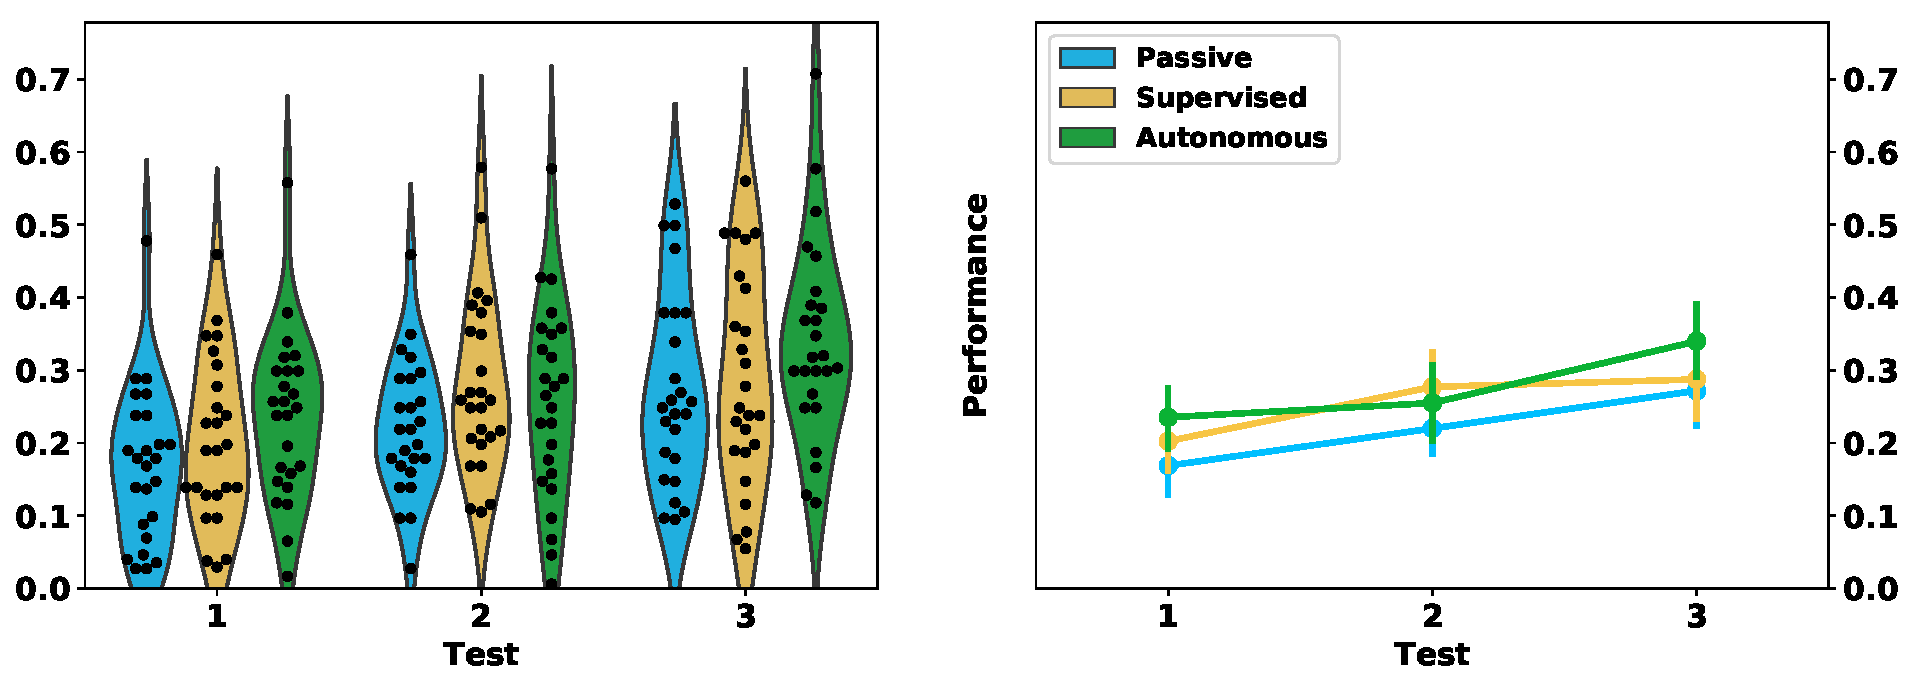
\includegraphics[width=1\linewidth]{perf.pdf}
	\centering
	\caption{Children's performance for the three tests: pretest, midtest and posttest for the three conditions.}
	\label{fig:performance}
\end{figure}

\begin{figure}[ht]
	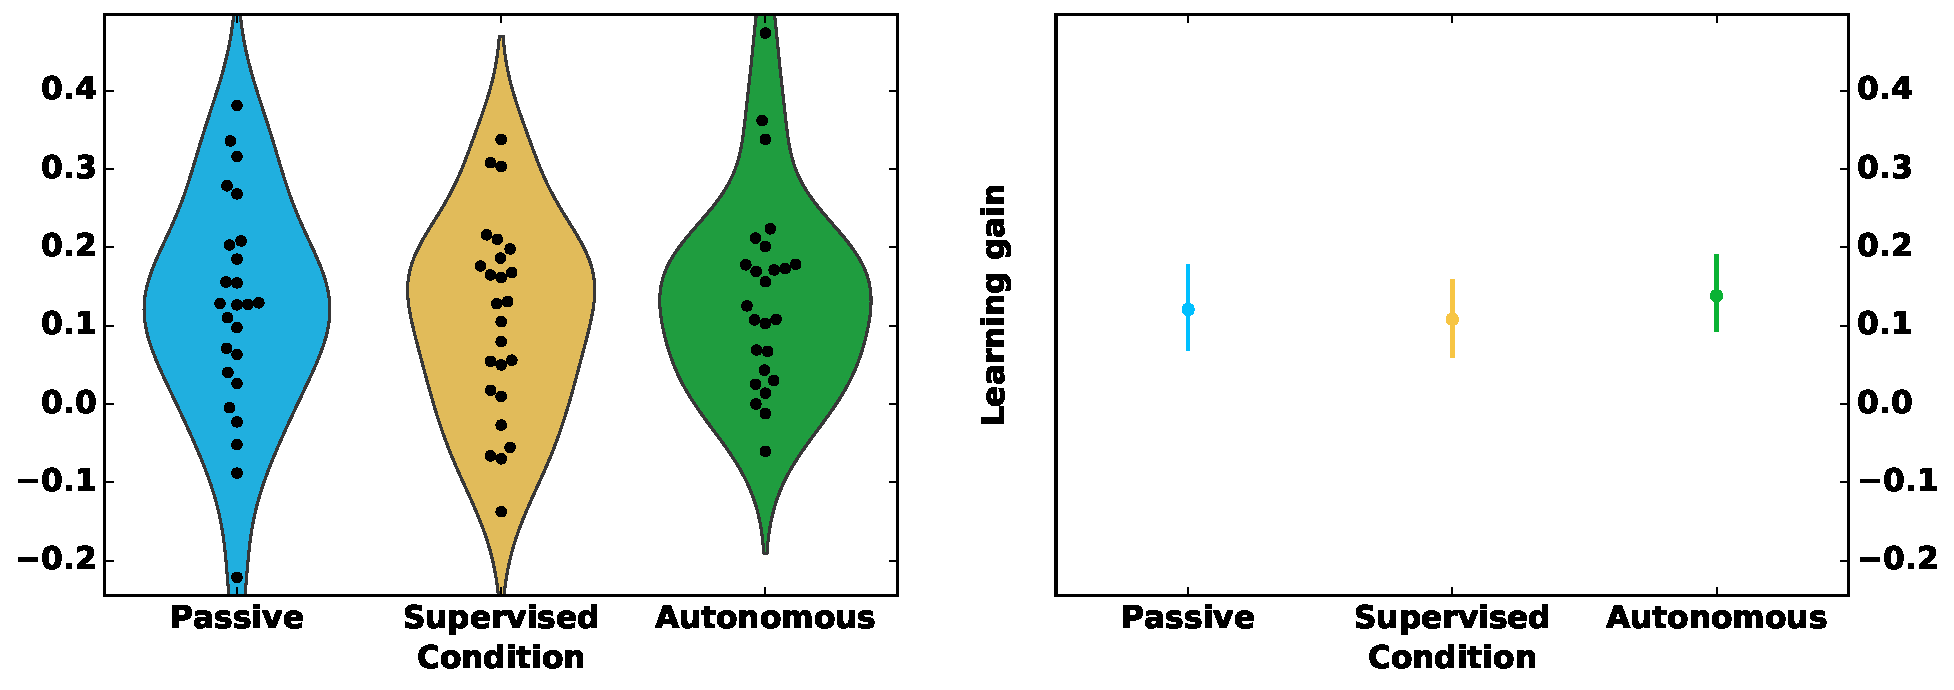
\includegraphics[width=1\linewidth]{learning.pdf}
	\centering
	\caption{Children's normalised learning gain after interacting with the robot for the three conditions.}
	\label{fig:learning}
\end{figure}

\paragraph{Game Metrics}

Figure \ref{fig:d_eat} shows the evolution of the number of different eating behaviour exhibited by the children across the four game sessions. A Bayesian mixed-ANOVA shows an impact of the condition on the number of different eating behaviour produced by the children in the game ($B=6.1$). Post-hoc tests show that there is no difference between the Supervised and the Autonomous conditions ($B=0.154$), whilst differences are observed between the Supervised and the Passive condition ($B=512$) and between the Autonomous and the Passive conditions ($B=246$). This indicates that the Supervised robot provided additional knowledge to the child during the game, allowing them to create more useful interactions between animals and their food, receiving more information from the game potentially helping them to learn. The Autonomous robot managed to recreate autonomously this effect without the presence of a human providing input.

\begin{figure}[ht]
	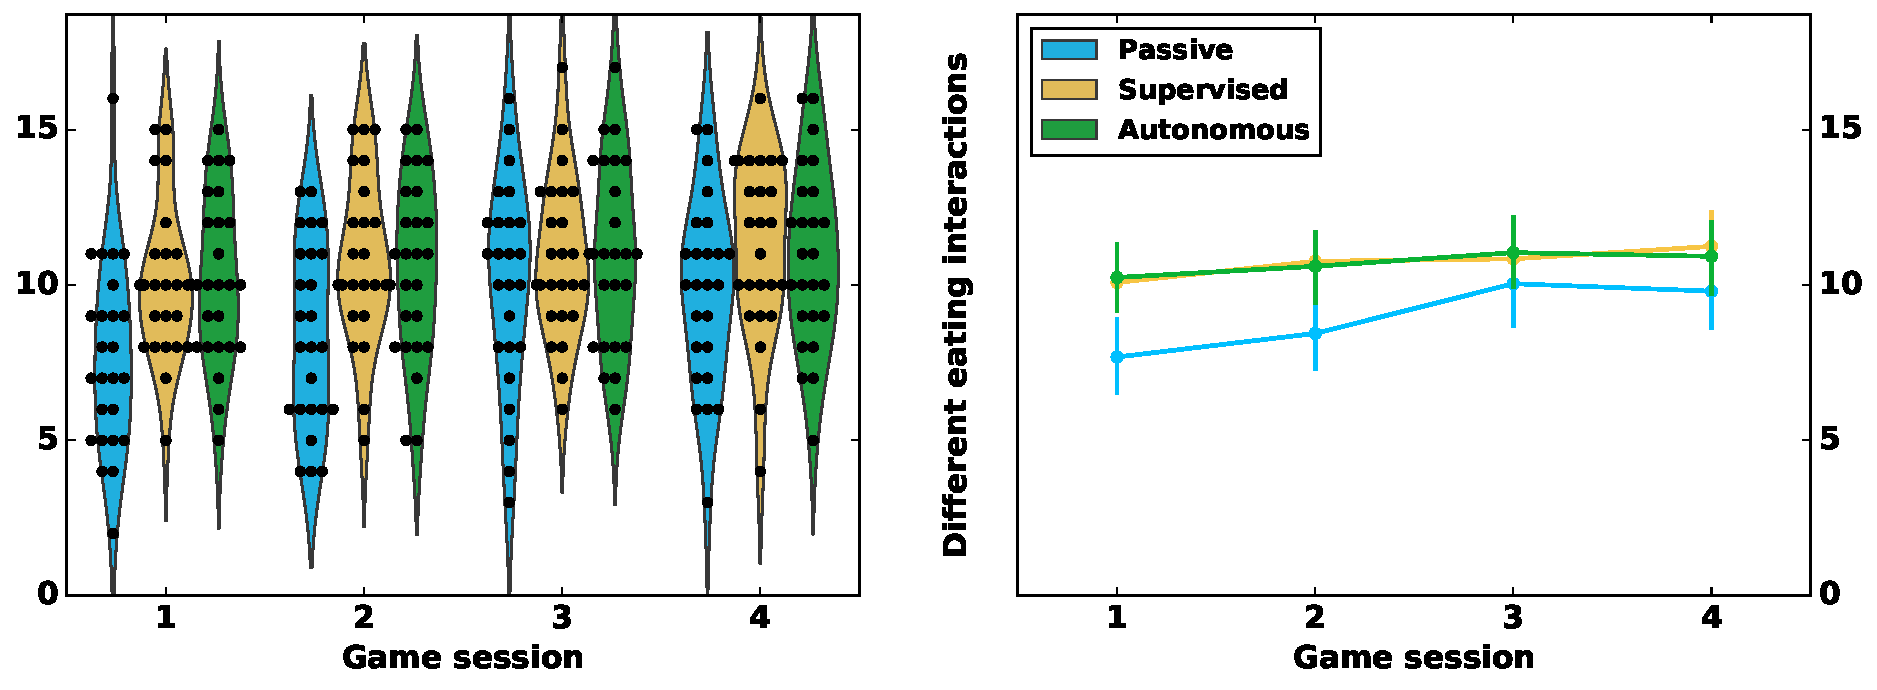
\includegraphics[width=1\linewidth]{d_eat.pdf}
	\centering
	\caption{Number of different eating behaviour for the four games for the three conditions.}
	\label{fig:d_eat}
\end{figure}

Figure \ref{fig:points} shows the evolution of the number of points achieved by the children across the four game sessions. A Bayesian mixed-ANOVA shows an impact of the condition on the number of points achieved by the children in the game ($B=10.2$). Post-hoc tests show a strong difference between the Passive and the Supervised conditions ($B=5.1$x$10^4$) and differences between the Supervised and the Autonomous conditions ($B=5.2$) and the Autonomous and the Passive condition ($B=5.9$). This indicates that when the robot was supervised, it allowed children to achieved more points than a  passive robot. And a similar effect is observed when the robot is autonomous, however the autonomous robot did not manage to reach the same efficiency as the supervised robot in helping the children to achieve a high score in the game.

\begin{figure}[ht]
	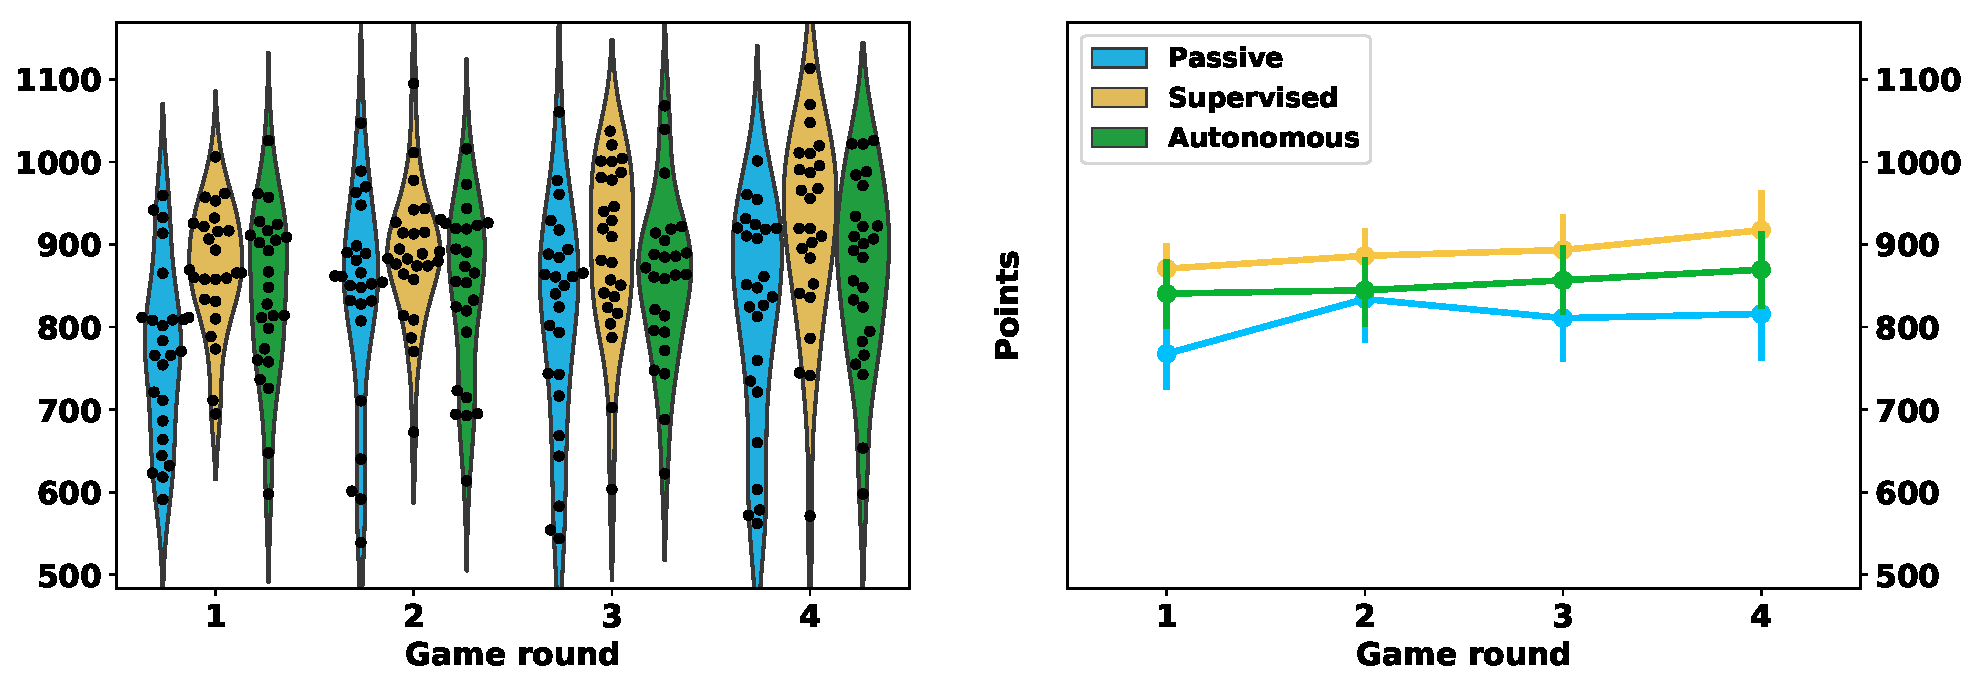
\includegraphics[width=1\linewidth]{points.pdf}
	\centering
	\caption{Points achieved by the children in each game session for the three conditions.}
	\label{fig:points}
\end{figure}

Figure \ref{fig:time} shows the evolution of interaction time across the four game sessions. A Bayesian mixed-ANOVA shows is inconclusive on the impact of the condition on the interaction time in the game ($B=1.1$). However, post-hoc tests show that there is no difference between the Supervised and the Autonomous conditions ($B=0.287$), whilst differences are observed between the Supervised and the Passive condition ($B=118$) and a tendency of difference between the Autonomous and the Passive conditions ($B=2.9$). This indicates that the Supervised robot allowed children to be better at the game, allowing them to maintain animal alive longer than a Passive robot. And the autonomous robot learn a policy tending to replicate this effect and without exhibiting differences with the supervised one.

\begin{figure}[ht]
	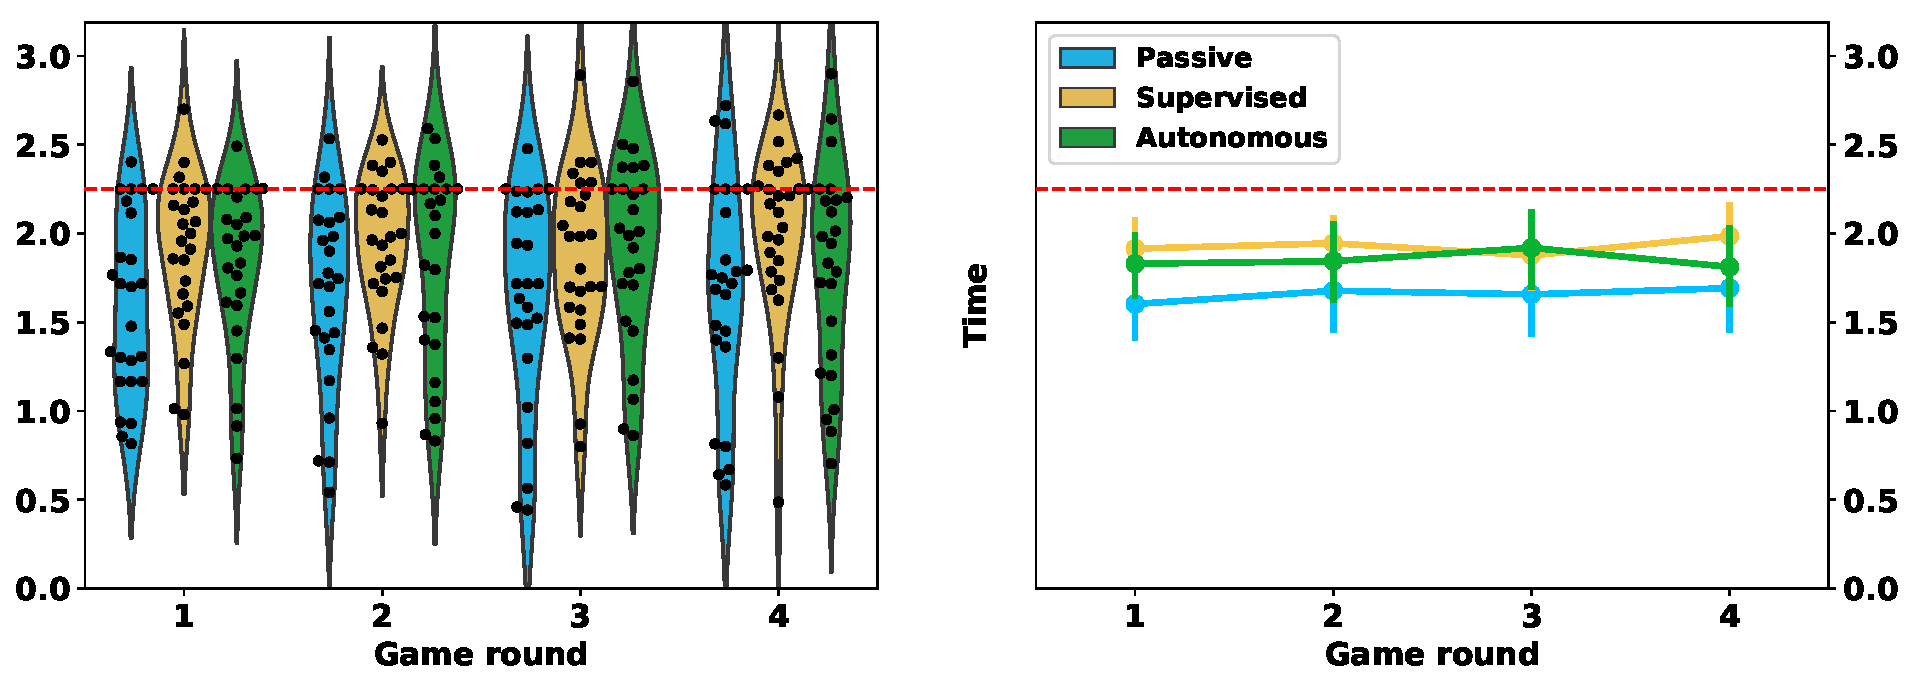
\includegraphics[width=1\linewidth]{time.pdf}
	\centering
	\caption{Interaction time for the four games for the three conditions.}
	\label{fig:time}
\end{figure}

These game metrics show that the action policy executed by the autonomous robot allows children to achieve similar results in the game than when the robot is supervised, and better results than when interacting with a passive robot. This provide support for H2 ("The robot reproduce the action policy demonstrated by the teacher enabling the child to achieve similar game metrics in autonomous and supervised condition but better than the passive condition"). However, children learned similarly in the three conditions, so these improvements in the game did not transfer to improvements in the test neither for the Supervised robot nor the Autonomous one. This does not support H1 ("The robot support child learning: learning gain in passive condition $<$ learning gain in autonomous condition $<$ learning gain in supervised condition")

\paragraph{Supervision}

Figure \ref{fig:tutoring_proposition} presents the reaction of the teacher to the robot's suggestions across all the supervised sessions. In average the teacher accepted 22.3\% of all the proposition of the robot (by enforcing the action, let it be executed or using the `Do it' button), which represents 35\% of the actions executed by the robot. This effect tends to be stable across the sessions. The teacher interaction pattern evolved overtime, such as by using mostly the `Cancel' button in the start then the `Skip' one, but in the end, the teacher used this two buttons mostly interchangeably even if the algorithm underlying reaction is different. Another observation is the evolution from using the auto-execution function to the `Do it' button once the teacher felt more comfortable in the supervision. The teacher reported three phases in her teaching: 

\begin{itemize}
	\item First sessions: she was not paying much attention to the suggestions, mostly trying to have the robot executing a correct action policy.
	\item Session 20 to around 65: she was paying more attention to the suggestions without giving them much credit.
	\item Last sessions: she started to trust the robot more but without ever trusting it totally.
\end{itemize}

\begin{figure}[ht]
	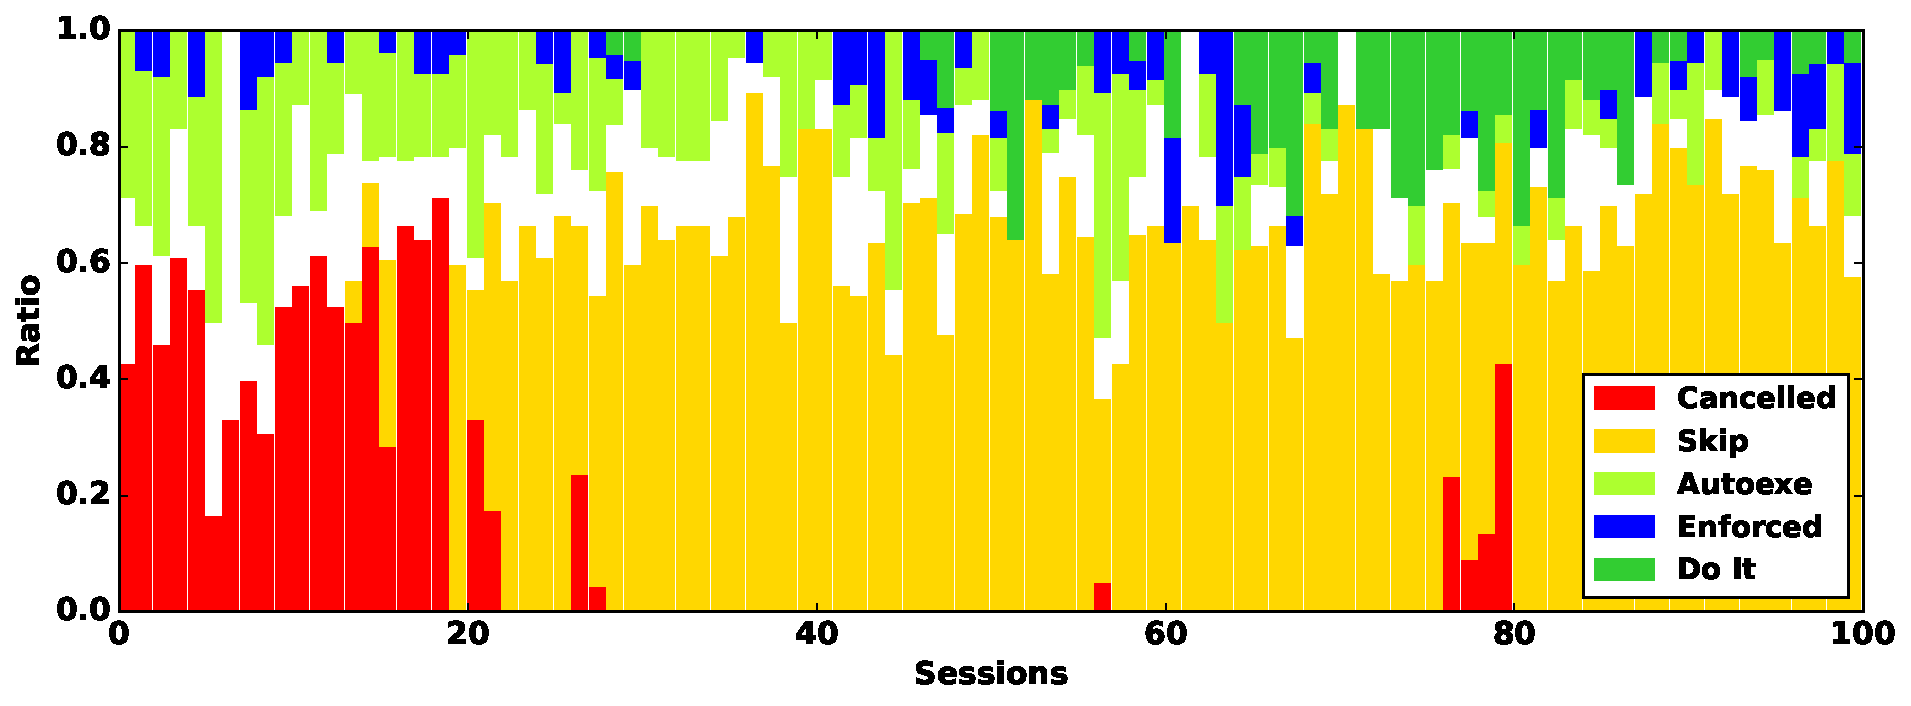
\includegraphics[width=1\linewidth]{propositions.pdf}
	\centering
	\caption{Teacher's reaction to the robot's propositions along the sessions.}
	\label{fig:tutoring_proposition}
\end{figure}


\begin{figure}[ht]
	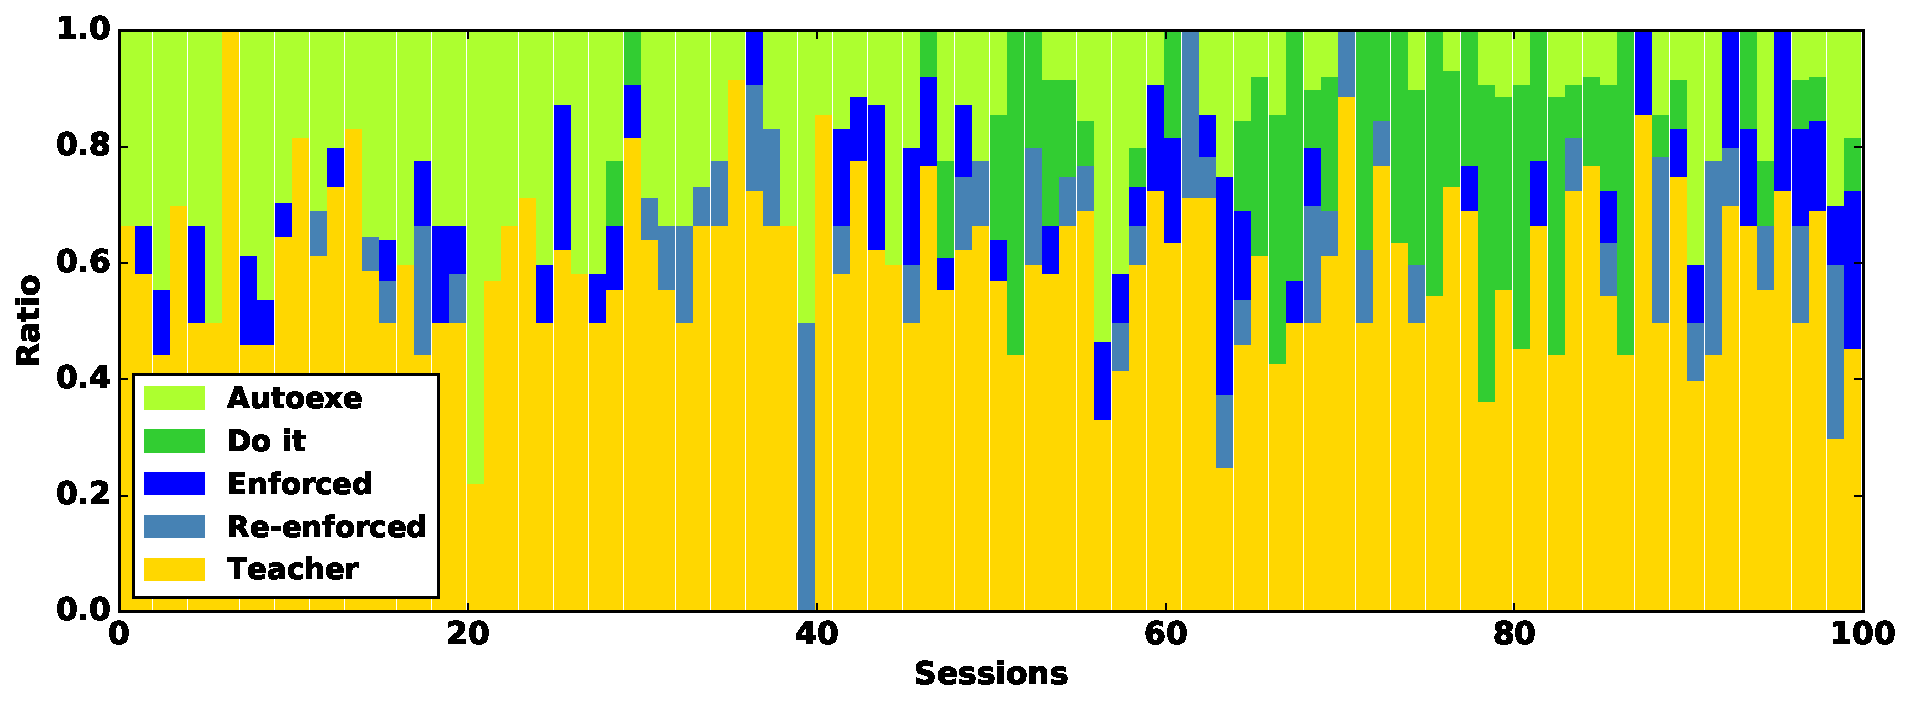
\includegraphics[width=1\linewidth]{selections.pdf}
	\centering
	\caption{Origin of the actions executed by the robot. Re-enforced actions indicates that an action has been selected after having been cancelled or skipped by the teacher.}
	\label{fig:tutoring_selection}
\end{figure}

Additional comments:
\begin{itemize}
	\item The robot proposed in average 58\% more actions than the number of actions selected by the teacher.
	\item As the time is continue and not discrete, the concept of correct actions is shifted, and actions selected by the teacher might have been proposed by the robot a fraction of second later without being counted as good proposition.
	\item The teacher often cancelled/skip actions directly as they arrived without taking time to analyse them (limitation of this implementation of SPARC).
	\item Evolution of teaching policy limits the potential of learning (not one single policy applied by the teacher, but an evolving one).
	\item Children are different, so the teacher tried to apply different action policy for each child.
\end{itemize}


\begin{figure}[ht]
	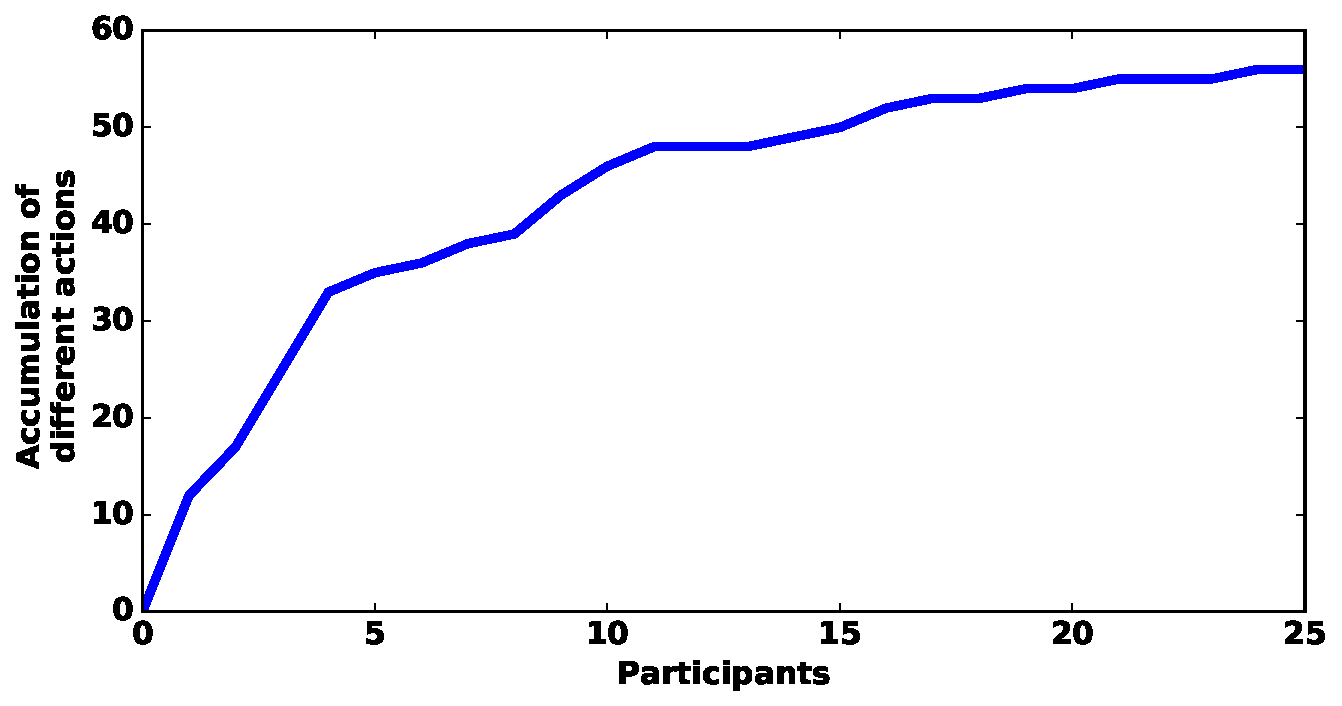
\includegraphics[width=.6\linewidth]{number_actions.pdf}
	\centering
	\caption{Accumulation of the number of different actions used by the teacher across the  participants.}
	\label{fig:tutoring_actions}
\end{figure}


\paragraph{Comparison of Policy}

Figures \ref{fig:tutoring_supervised_actions} and \ref{fig:tutoring_autonomous_actions} present the policies used by the teacher and the autonomous robot across their participants. It should be noted that participants in both conditions are different.


\begin{figure}[ht]
	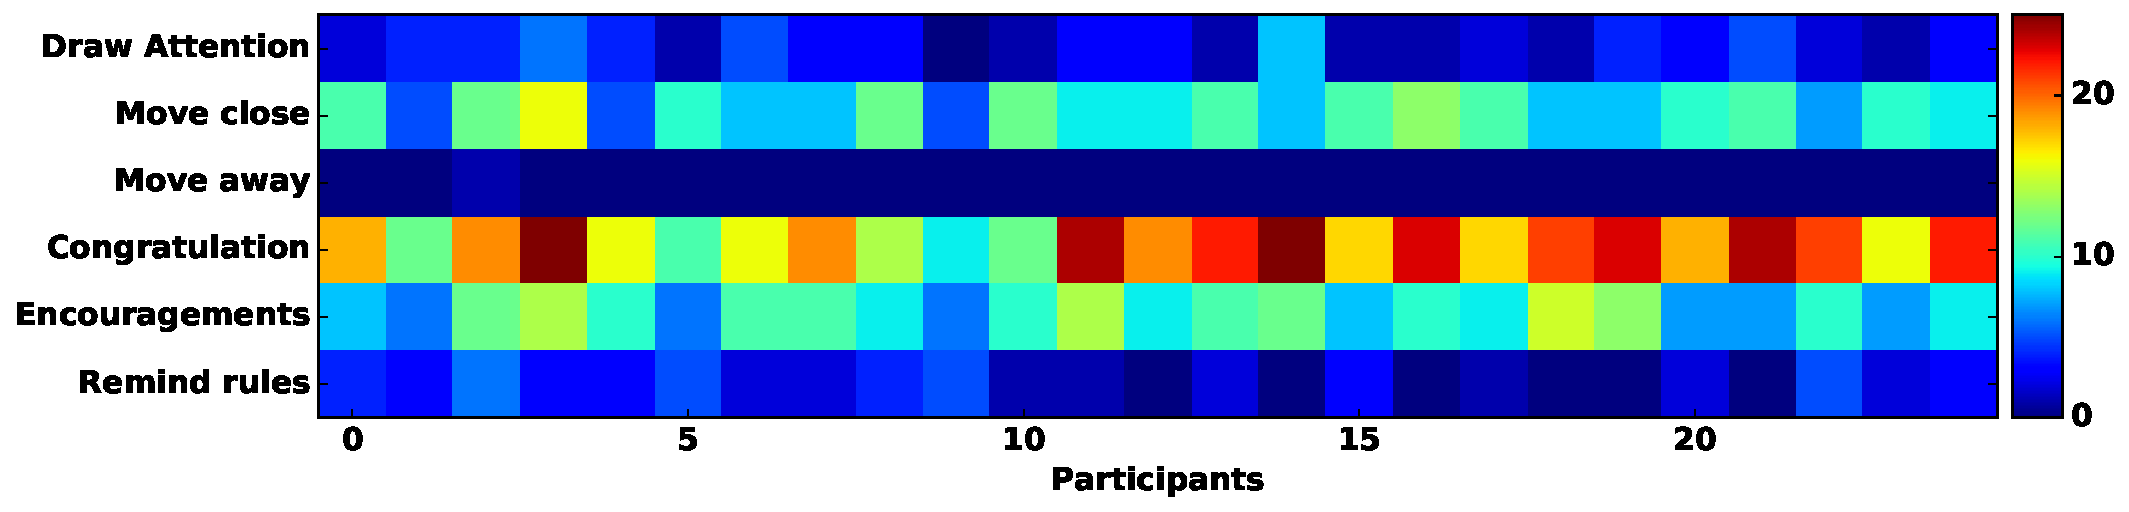
\includegraphics[width=1\linewidth]{supervised_actions.pdf}
	\centering
	\caption{Repartition of actions across the participants in the supervised condition.}
	\label{fig:tutoring_supervised_actions}
\end{figure}

\begin{figure}[ht]
	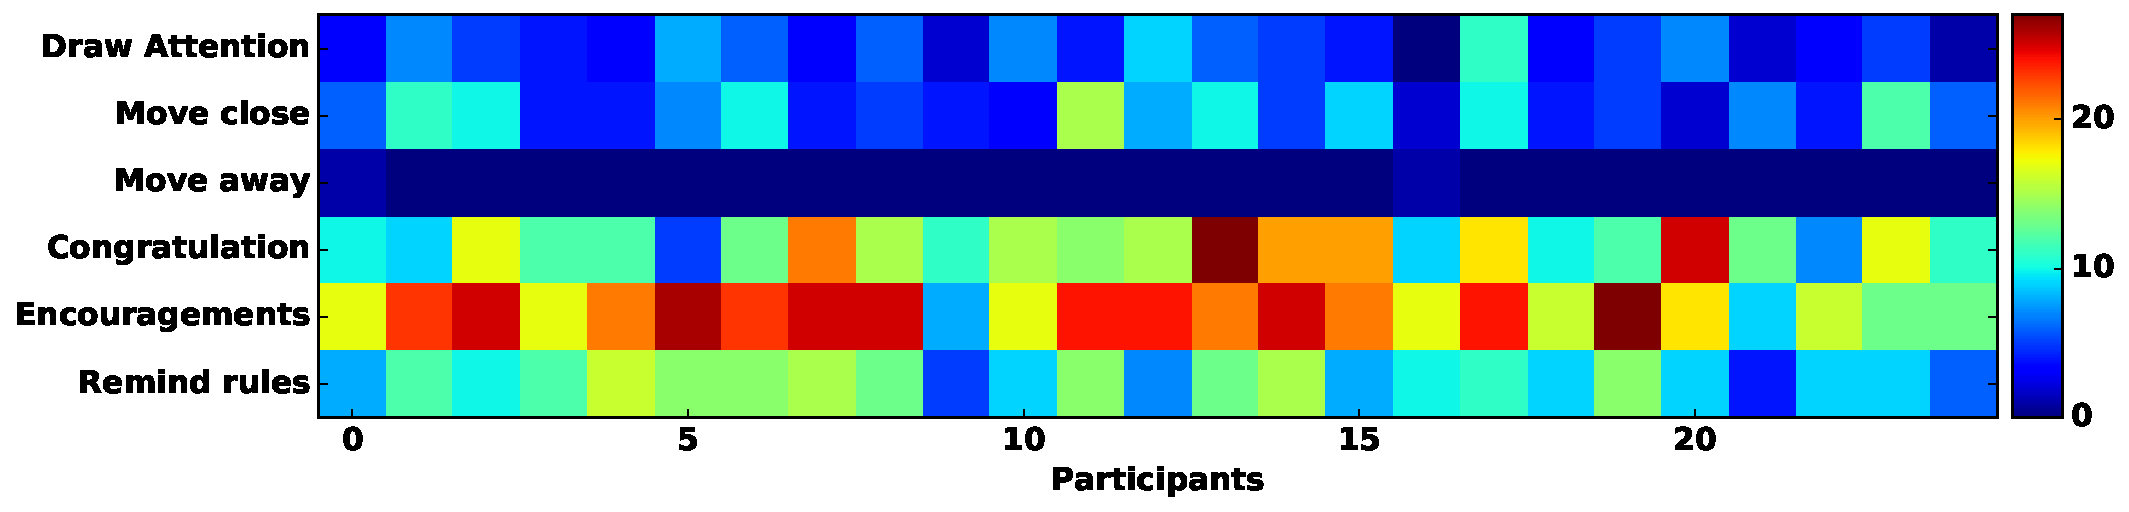
\includegraphics[width=1\linewidth]{autonomous_actions.pdf}
	\centering
	\caption{Repartition of actions across the participants in the autonomous condition.}
	\label{fig:tutoring_autonomous_actions}
\end{figure}

\begin{table}[ht]
	\centering
	\caption{Repartition of action in the policy for both conditions (in \%).}
	\label{tab:tutoring_policies}
	\begin{tabularx}{\textwidth}{@{}lYYYccY}\toprule
		& Draw \newline Attention & Move \newline close & Move \newline away & Congratulation & Encouragements & Remind \newline rules \\
		\midrule
		Supervised & 6.6  & 22.2 & 0.1 & 43.1 & 22.7 & 5.3 \\
		Autonomous & 8.5 & 11.8 & 0.1 & 25.4 & 35.2 & 18.9\\
		\bottomrule
	\end{tabularx}
\end{table}

\section{Discussion}

\section{Summary}

